\documentclass[aspectratio=169,10pt]{beamer}

% Theme
\usetheme{Madrid}
\useinnertheme{rounded}
\setbeamertemplate{navigation symbols}{}
\setbeamertemplate{caption}[numbered]
\setbeameroption{hide notes}

% Packages
\usepackage[T1]{fontenc}
\usepackage[utf8]{inputenc}
\usepackage{lmodern}
\usepackage{amsmath,amssymb}
\usepackage{booktabs}
\usepackage{array}
\usepackage{graphicx}
\usepackage{xcolor}
\usepackage{tikz}
\usetikzlibrary{positioning,arrows.meta,fit,calc,backgrounds,shapes.geometric}
\usepackage{ragged2e}
\usepackage{makecell}

% Colors - middle ground between clean academic and visual polish
\definecolor{DeepBlue}{HTML}{0D1B2A}
\definecolor{MidBlue}{HTML}{1B4F72}
\definecolor{AccentBlue}{HTML}{2E86AB}
\definecolor{SoftBlue}{HTML}{EAF2F8}
\definecolor{SoftGreen}{HTML}{E8F6EF}
\definecolor{SoftGold}{HTML}{FFF3CD}
\definecolor{WarmGold}{HTML}{E8A838}
\definecolor{SoftRed}{HTML}{FDEDEC}
\definecolor{MutedGray}{HTML}{4D5656}

\setbeamercolor{palette primary}{bg=DeepBlue,fg=white}
\setbeamercolor{palette secondary}{bg=MidBlue,fg=white}
\setbeamercolor{palette tertiary}{bg=AccentBlue,fg=white}
\setbeamercolor{structure}{fg=MidBlue}
\setbeamercolor{frametitle}{bg=SoftBlue,fg=MidBlue}
\setbeamercolor{title}{fg=DeepBlue}
\setbeamercolor{subtitle}{fg=MidBlue}
\setbeamercolor{block title}{bg=MidBlue!14,fg=MidBlue}
\setbeamercolor{block body}{bg=MidBlue!4,fg=black}
\setbeamercolor{block title alerted}{bg=WarmGold!90,fg=DeepBlue}
\setbeamercolor{block body alerted}{bg=SoftGold,fg=black}
\setbeamercolor{exampleblock title}{bg=AccentBlue!18,fg=MidBlue}
\setbeamercolor{exampleblock body}{bg=AccentBlue!5,fg=black}

% Roomier footline: includes authors and avoids cropped text
\setbeamertemplate{footline}{%
  \leavevmode%
  \hbox{%
  \begin{beamercolorbox}[wd=.34\paperwidth,ht=3.2ex,dp=1.2ex,leftskip=0.8em]{palette primary}%
    \usebeamerfont{author in head/foot}\scriptsize\vphantom{Ag} Nour Gaser \& Mohamed Wael
  \end{beamercolorbox}%
  \begin{beamercolorbox}[wd=.48\paperwidth,ht=3.2ex,dp=1.2ex,center]{palette primary}%
    \usebeamerfont{title in head/foot}\scriptsize\vphantom{Ag} Tri-CAN for Egyptian Arabic MER
  \end{beamercolorbox}%
  \begin{beamercolorbox}[wd=.18\paperwidth,ht=3.2ex,dp=1.2ex,rightskip=0.8em]{palette secondary}%
    \hfill\usebeamerfont{date in head/foot}\scriptsize\vphantom{Ag} \insertframenumber/\inserttotalframenumber
  \end{beamercolorbox}}%
  \vskip0pt%
}

\setbeamersize{text margin left=0.55cm,text margin right=0.55cm}
\setbeamerfont{title}{size=\Large,series=\bfseries}
\setbeamerfont{subtitle}{size=\normalsize}
\setbeamerfont{frametitle}{size=\large,series=\bfseries}
\setbeamerfont{block title}{size=\normalsize,series=\bfseries}
\setbeamerfont{block body}{size=\small}
\setbeamerfont{itemize/enumerate body}{size=\small}
\setbeamerfont{itemize/enumerate subbody}{size=\footnotesize}

% Commands
\newcommand{\term}[1]{\textbf{\textcolor{MidBlue}{#1}}}
\newcommand{\gold}[1]{\textbf{\textcolor{WarmGold!85!black}{#1}}}
\newcommand{\muted}[1]{\textcolor{MutedGray}{#1}}
\newcommand{\source}[1]{\vspace{0.05cm}\hfill{\scriptsize\textcolor{MutedGray}{#1}}}
\newcommand{\keytake}[1]{\vspace{0.3em}{\small #1}}

% Metadata
\title[Tri-CAN for Egyptian Arabic MER]{Enhancing Egyptian Arabic Multimodal Emotion Recognition via Cross-Modal Attention}
\subtitle{Research Project II Proposal: Tri-Modal Cross-Attention Network (Tri-CAN)}
\author[N. Gaser \& M. Wael]{Nour Gaser \and Mohamed Wael}
\institute[GIU]{German International University\\Research Project I - Winter 2026}
\date{February 2026}

\begin{document}

% 1
{\setbeamertemplate{footline}{}
\setbeamercolor{background canvas}{bg=DeepBlue}
\begin{frame}[plain]
\vspace{0.75cm}
\begin{center}
{\color{white}\LARGE\bfseries Enhancing Egyptian Arabic\\[0.15cm]
Multimodal Emotion Recognition}\\[0.35cm]
{\color{AccentBlue!25!white}\Large via Cross-Modal Attention}\\[0.65cm]
\begin{beamercolorbox}[rounded=true,sep=0.35cm,wd=0.78\linewidth]{block body}
\centering
\small Can feature-level interaction between \term{text}, \term{audio}, and \term{video} improve Egyptian Arabic emotion recognition beyond gated late fusion?
\end{beamercolorbox}
\vspace{0.65cm}
{\color{white}\normalsize Nour Gaser \quad \& \quad Mohamed Wael}\\[0.15cm]
{\color{white!70}\small German International University - Research Project I - Winter 2026}
\end{center}
\note{Open with the core question. Do not introduce all technical details yet.}
\end{frame}
\setbeamercolor{background canvas}{bg=white}
}

% 2
\begin{frame}[t]{Roadmap: From Problem to Experiment}
\begin{columns}[T,onlytextwidth]
\column{0.33\linewidth}
\begin{block}{1. Context}
\begin{itemize}
  \item How the literature was reviewed
  \item Multimodal emotion recognition
  \item Egyptian Arabic and sarcasm
  \item EGY-MER dataset constraints
\end{itemize}
\end{block}
\column{0.33\linewidth}
\begin{block}{2. Proposed method}
\begin{itemize}
  \item Why late fusion is limited
  \item Tri-CAN architecture
  \item Cross-attention, LoRA, focal loss
\end{itemize}
\end{block}
\column{0.33\linewidth}
\begin{block}{3. Experiment}
\begin{itemize}
  \item Baselines and ablations
  \item Metrics and validation
  \item VAD-avatar idea as future work
\end{itemize}
\end{block}
\end{columns}
\vspace{0.5cm}
\keytake{The question is whether letting the modalities interact helps with Egyptian Arabic sarcasm and cases where words and delivery disagree.}
\note{Tell the supervisor you will keep the math minimal but show enough detail to justify the architecture.}
\end{frame}

% 2a
\begin{frame}[t]{How the Literature Was Reviewed}
\begin{columns}[T,onlytextwidth]
\column{0.56\linewidth}
\centering
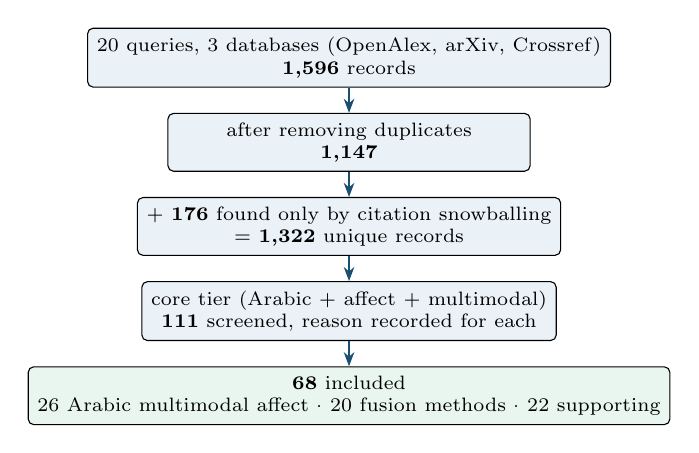
\begin{tikzpicture}[font=\scriptsize, >={Stealth[length=1.8mm]},
  st/.style={draw,rounded corners=2pt,fill=SoftBlue,align=center,minimum width=4.6cm,minimum height=0.62cm}]
\node[st] (q) {20 queries, 3 databases (OpenAlex, arXiv, Crossref)\\\textbf{1,596} records};
\node[st,below=0.32cm of q] (d) {after removing duplicates\\\textbf{1,147}};
\node[st,below=0.32cm of d] (s) {+ \textbf{176} found only by citation snowballing\\= \textbf{1,322} unique records};
\node[st,below=0.32cm of s] (c) {core tier (Arabic + affect + multimodal)\\\textbf{111} screened, reason recorded for each};
\node[st,below=0.32cm of c,fill=SoftGreen] (i) {\textbf{68} included\\26 Arabic multimodal affect \textperiodcentered{} 20 fusion methods \textperiodcentered{} 22 supporting};
\draw[->,MidBlue] (q)--(d); \draw[->,MidBlue] (d)--(s); \draw[->,MidBlue] (s)--(c); \draw[->,MidBlue] (c)--(i);
\end{tikzpicture}
\column{0.41\linewidth}
\begin{block}{Protocol}
\begin{itemize}
  \item Fixed before searching; covers everything up to 31 July 2026
  \item Snowballing in both directions from 4 seed papers: EGY-MER, Ar-MuSA, UniTextFusion, MulT
  \item Every record and decision is in the tracking spreadsheet (\texttt{RP1\_paper\_tracking.xlsx})
\end{itemize}
\end{block}
\begin{block}{Limitations}
\begin{itemize}
  \item Screening at title and abstract level
  \item Semantic Scholar needed an API key we did not have
\end{itemize}
\end{block}
\end{columns}
\note{If asked about tools: the search scripts were written with Claude Code, and it did the first screening pass, which we then reviewed. All bibliographic details come from the databases or publishers, not typed in by hand or by a model. This is also written in Section 2.1 of the report.}
\end{frame}

% 2b
\begin{frame}[t]{What the Review Found in 2026}
\begin{columns}[T,onlytextwidth]
\column{0.52\linewidth}
\begin{block}{Attention models on Arabic sentiment}
\centering\small
\begin{tabular}{@{}lc@{}}
\toprule
Ar-MuSA, 3-class sentiment & F1 \\
\midrule
UniTextFusion (2025) & 0.71 \\
Tri-modal early fusion (2026) & 0.776 \\
GCMA-Net, gated cross-modal attention (2026) & 0.802 \\
Directional semantic enhancement (2026) & 0.899 \\
\bottomrule
\end{tabular}
\end{block}
\column{0.44\linewidth}
\begin{block}{Arabic emotion: no follow-up yet}
\begin{itemize}
  \item All of this work is on Ar-MuSA and sentiment polarity.
  \item EGY-MER (7 emotions, Egyptian Arabic) has no published follow-up; its 0.519 baseline is untouched.
  \item New emotion corpora exist, e.g.\ MORAD: 2,325 Moroccan videos with the same 7 emotions.
\end{itemize}
\end{block}
\end{columns}
\vspace{0.3cm}
\small This changed the fourth gap in the proposal: the mechanism is no longer new to Arabic, but the task is.
\source{Khaled et al., 2025; Ben Cheikhi et al., 2026 (three papers); Atou et al., 2026}
\note{Be upfront: this was found by our own review and it removed part of the original novelty claim. The report's Section 2.4.5 covers these papers.}
\end{frame}

% 3
\begin{frame}[t]{Motivation: Why Egyptian Arabic Multimodal Emotion?}
\begin{columns}[T,onlytextwidth]
\column{0.51\linewidth}
\begin{block}{Why multimodal?}
Human emotion is not carried by text alone.
\vspace{0.25em}
\begin{itemize}
  \item \term{Text}: words and lexical sentiment
  \item \term{Audio}: pitch, tone, pauses, intensity
  \item \term{Video}: facial expression, eye movement, gestures
\end{itemize}
\end{block}
\begin{alertblock}{Recurring example}
\centering
\Large ``Ah, momtaz!''\\[-0.1cm]
\normalsize\muted{``Oh, excellent!''}
\end{alertblock}
\column{0.46\linewidth}
\begin{block}{Why Egyptian Arabic?}
\begin{itemize}
  \item Dialectal Arabic is under-resourced compared with English.
  \item Egyptian Arabic has informal spelling, code-switching, and cultural expressions.
  \item Sarcasm often creates \term{polarity contradiction}: positive words, negative intent.
\end{itemize}
\end{block}
\begin{exampleblock}{Presentation intuition}
The same phrase can be praise or criticism depending on flat tone, mocking voice, or an eye-roll.
\end{exampleblock}
\end{columns}
\source{Rahma et al., 2023; Hussein et al., 2025}
\note{Use the phrase as the single example throughout the talk to avoid repetition.}
\end{frame}

% 4
\begin{frame}[t]{Dataset Context: From Scarcity to EGY-MER}
\begin{columns}[T,onlytextwidth]
\column{0.58\linewidth}
\begin{block}{Arabic multimodal dataset landscape}
\centering
\scriptsize
\begin{tabular}{@{}>{\centering\arraybackslash}p{0.28\linewidth}>{\centering\arraybackslash}p{0.28\linewidth}>{\centering\arraybackslash}p{0.28\linewidth}@{}}
\toprule
\textbf{AMMD} & \textbf{EGY-MER} & \textbf{Ar-MuSA} \\
\midrule
2019 & 2025 & 2025 \\
40 videos / 830 utt. & 363 segments & 8,700 samples \\
MSA + Gulf + Levantine & Egyptian Arabic only & Egyptian + MSA \\
\bottomrule
\end{tabular}
\end{block}
\begin{block}{Primary dataset: EGY-MER}
\begin{itemize}
  \item 363 clean single-speaker Egyptian Arabic segments
  \item Sources: talk shows and dramas
  \item Modalities: transcript, audio, video
  \item Labels: 7 emotion classes
\end{itemize}
\end{block}
\column{0.39\linewidth}
\begin{alertblock}{Two practical constraints}
\begin{enumerate}
  \item \textbf{Small data}: 363 samples is risky for large models.
  \item \textbf{Class imbalance}: Fear and Surprise each constitute less than 4\%.
\end{enumerate}
\end{alertblock}
\begin{exampleblock}{Why this shapes the method}
The proposal needs both a stronger fusion mechanism \emph{and} a training strategy that avoids overfitting.
\end{exampleblock}
\end{columns}
\source{Alqarafi et al., 2019; Hussein et al., 2025; Khaled et al., 2025b}
\note{Emphasize that EGY-MER is valuable but small, which justifies LoRA and cross-validation later.}
\end{frame}

% 5
\begin{frame}[t]{Fusion Techniques: Where the Gap Appears}
\begin{center}
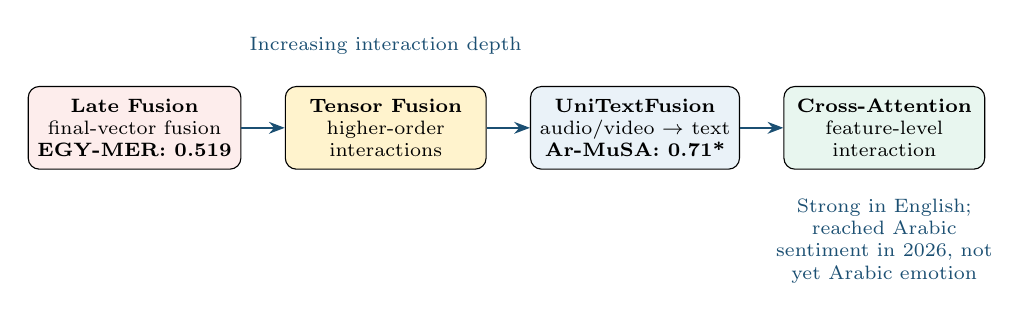
\begin{tikzpicture}[font=\scriptsize, >={Stealth[length=2mm]}, box/.style={draw,rounded corners,align=center,minimum width=2.55cm,minimum height=1.05cm}]
\node[box,fill=SoftRed] (late) {\textbf{Late Fusion}\\final-vector fusion\\\textbf{EGY-MER: 0.519}};
\node[box,fill=SoftGold,right=0.55cm of late] (tensor) {\textbf{Tensor Fusion}\\higher-order\\interactions};
\node[box,fill=SoftBlue,right=0.55cm of tensor] (uni) {\textbf{UniTextFusion}\\audio/video\ $\rightarrow$ text\\\textbf{Ar-MuSA: 0.71*}};
\node[box,fill=SoftGreen,right=0.55cm of uni] (cross) {\textbf{Cross-Attention}\\feature-level\\interaction};
\draw[->,thick,MidBlue] (late) -- (tensor);
\draw[->,thick,MidBlue] (tensor) -- (uni);
\draw[->,thick,MidBlue] (uni) -- (cross);
\node[above=0.28cm of tensor,align=center,MidBlue] {Increasing interaction depth};
\node[below=0.25cm of cross,align=center,text width=2.9cm,MidBlue] {Strong in English; reached Arabic sentiment in 2026, not yet Arabic emotion};
\end{tikzpicture}
\end{center}
\vspace{0.3cm}
\begin{columns}[T,onlytextwidth]
\column{0.48\linewidth}
\begin{block}{What late fusion does well}
\begin{itemize}
  \item Modular and easier to train
  \item Each encoder can be optimized independently
\end{itemize}
\end{block}
\column{0.48\linewidth}
\begin{alertblock}{What it misses}
A scalar fusion weight cannot ask: \emph{which exact audio moment or facial frame explains this specific word?}
\end{alertblock}
\end{columns}
\source{Hussein et al., 2025; Khaled et al., 2025a; Tsai et al., 2019. *Not directly comparable.}
\note{This is the bridge from literature review to the gap. Do not attack late fusion; call it a reasonable baseline with limits.}
\end{frame}

% 6
\begin{frame}[t]{Why Late Fusion Struggles with Sarcasm}
\begin{columns}[T,onlytextwidth]
\column{0.56\linewidth}
\begin{center}
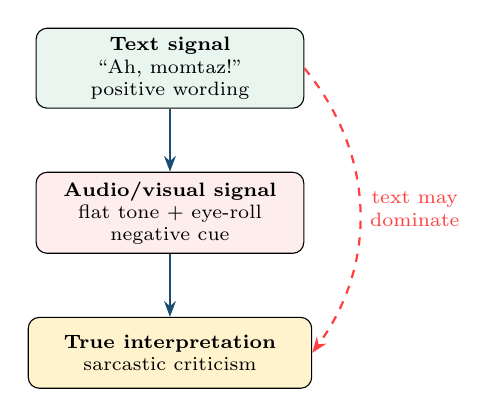
\begin{tikzpicture}[font=\scriptsize, >={Stealth[length=2mm]}]
\node[draw,rounded corners,fill=SoftGreen,align=center,minimum width=3.4cm,minimum height=1cm] (text) {\textbf{Text signal}\\``Ah, momtaz!''\\positive wording};
\node[draw,rounded corners,fill=SoftRed,align=center,minimum width=3.4cm,minimum height=1cm,below=0.8cm of text] (av) {\textbf{Audio/visual signal}\\flat tone + eye-roll\\negative cue};
\node[draw,rounded corners,fill=SoftGold,align=center,minimum width=3.6cm,minimum height=0.9cm,below=0.8cm of av] (truth) {\textbf{True interpretation}\\sarcastic criticism};
\draw[->,thick,MidBlue] (text) -- (av);
\draw[->,thick,MidBlue] (av) -- (truth);
\draw[->,thick,dashed,red!75] (text.east) to[bend left=38] node[right,align=center]{text may\\dominate} (truth.east);
\end{tikzpicture}
\end{center}
\column{0.41\linewidth}
\begin{block}{The independence assumption}
Late fusion combines already-compressed modality vectors at the final decision stage.
\end{block}
\begin{alertblock}{Failure mode}
If text is the strongest unimodal predictor, contradictory tone/face cues can be underused.
\end{alertblock}
\begin{exampleblock}{Research implication}
The architecture should model \term{incongruence} between modalities, not only aggregate them.
\end{exampleblock}
\end{columns}
\note{This slide should feel like the problem statement, not just another definition.}
\end{frame}

% 7
\begin{frame}[t]{Four Gaps Driving the Proposal}
\begin{columns}[T,onlytextwidth]
\column{0.49\linewidth}
\begin{block}{1. Independence assumption}
Late fusion treats text/audio/video as mostly independent until classification.
\end{block}
\begin{block}{2. Sarcasm bottleneck}
Egyptian Arabic often relies on contradiction between positive wording and negative tone/face.
\end{block}
\column{0.49\linewidth}
\begin{block}{3. Data efficiency}
EGY-MER has 363 samples across 7 classes, so full end-to-end training risks overfitting.
\end{block}
\begin{block}{4. Arabic \emph{emotion} recognition}
Cross-modal attention reached Arabic sentiment in 2026, but only on Ar-MuSA's 3-class polarity. Nobody has tried it on 7-class Arabic emotion, where EGY-MER's baseline (0.519) is still unchallenged.
\end{block}
\end{columns}
\vspace{0.25cm}
\keytake{Tri-CAN is aimed at all four: modality interaction, sarcasm, small data, and emotion rather than sentiment.}
\source{Tsai et al., 2019; Hussein et al., 2025; Rahma et al., 2023; Ben Cheikhi et al., 2026}
\note{Gap 4 was originally ``cross-attention has never been tried on Arabic''. Our own systematic search found it was done in 2026 on Ar-MuSA, so the gap is now narrower: emotion, not sentiment. The report was corrected the same way.}
\note{This is a good slide to slow down and make the research contribution explicit.}
\end{frame}

% 8
\begin{frame}[t]{Proposed Architecture: Tri-CAN}
\begin{columns}[T,onlytextwidth]
\column{0.59\linewidth}
\centering
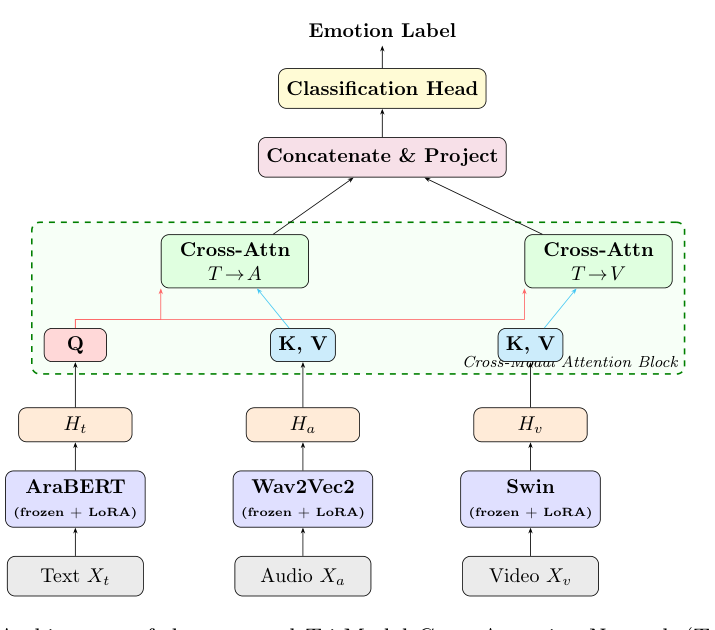
\includegraphics[width=\linewidth,height=0.70\textheight,keepaspectratio]{../report/trican_architecture.png}
\column{0.38\linewidth}
\begin{block}{Core idea}
Text actively \term{queries} audio and video before classification.
\end{block}
\begin{block}{Encoders}
\begin{itemize}
  \item Text: AraBERT
  \item Audio: Wav2Vec2
  \item Video: Swin Transformer
\end{itemize}
\end{block}
\begin{alertblock}{Difference from late fusion}
Instead of fusing only final vectors, Tri-CAN performs feature-level alignment between words and non-verbal cues.
\end{alertblock}
\end{columns}
\note{Point bottom-to-top: inputs, encoders, cross-attention block, classifier.}
\end{frame}

% 9
\begin{frame}[t]{Cross-Attention Intuition: Queries, Keys, Values}
\begin{columns}[T,onlytextwidth]
\column{0.32\linewidth}
\begin{block}{Query (Q)}
The question being asked.\\[0.25em]
\textbf{Here:} text asks which audio/video cues are relevant.
\end{block}
\column{0.32\linewidth}
\begin{block}{Keys (K)}
Searchable descriptors of audio/video moments.\\[0.25em]
Examples: pause, shout, sarcastic laugh, eye-roll.
\end{block}
\column{0.32\linewidth}
\begin{block}{Values (V)}
The actual information retrieved once relevance is known.\\[0.25em]
These enrich the text representation.
\end{block}
\end{columns}
\vspace{0.35cm}
\begin{exampleblock}{Search-engine analogy}
Query = what you type; Keys = searchable page titles/descriptors; Values = page contents returned.
\end{exampleblock}
\begin{alertblock}{Important nuance}
Cross-attention is not merely ``merging features''; it is one modality dynamically retrieving relevant information from another.
\end{alertblock}
\note{Use the Google Search analogy. This is the clearest explanation for Q/K/V.}
\end{frame}

% 10
\begin{frame}[t]{The Attention Equation}
\begin{block}{Scaled dot-product attention}
\centering
\Large
$\displaystyle \text{Attention}(Q,K,V)=\underbrace{\text{softmax}\left(\frac{\overbrace{QK^T}^{\text{similarity}}}{\sqrt{d_k}}\right)}_{\text{attention weights}}\;\underbrace{V}_{\text{retrieved information}}$
\end{block}
\vspace{0.25cm}
\begin{columns}[T,onlytextwidth]
\column{0.48\linewidth}
\begin{block}{For text-to-audio}
\small
$Q = H_tW_Q$ comes from text.\\
$K = H_aW_K$ and $V = H_aW_V$ come from audio.
\vspace{0.2cm}
\begin{center}
\term{Question:} Which audio frames explain this word?
\end{center}
\end{block}
\column{0.48\linewidth}
\begin{block}{For text-to-video}
\small
Same equation, but audio features $H_a$ are replaced by visual features $H_v$.
\vspace{0.2cm}
\begin{center}
\term{Question:} Which visual frames explain this word?
\end{center}
\end{block}
\end{columns}
\note{Say: the only math you need to remember is similarity -> weights -> retrieve information.}
\end{frame}

% 11
\begin{frame}[t]{Training Strategy: Frozen Encoders + LoRA}
\begin{columns}[T,onlytextwidth]
\column{0.49\linewidth}
\begin{block}{Why not fully fine-tune everything?}
\begin{itemize}
  \item AraBERT, Wav2Vec2, and Swin are large pretrained models.
  \item EGY-MER has only 363 samples.
  \item Full fine-tuning would be expensive and could memorize the dataset.
\end{itemize}
\end{block}
\begin{exampleblock}{Frozen means}
The original pretrained weights are kept fixed; the encoder acts as a strong feature extractor.
\end{exampleblock}
\column{0.48\linewidth}
\begin{block}{LoRA: small trainable correction}
Instead of updating all weights $W$:
\[
W' = W + \Delta W = W + BA
\]
where $B \in \mathbb{R}^{d \times r}$, $A \in \mathbb{R}^{r \times k}$, and $r \ll d$.
\end{block}
\begin{alertblock}{Why it fits this project}
\begin{itemize}
  \item Up to around 98\% fewer trainable parameters
  \item More feasible on 12--16 GB VRAM
  \item LoRA ranks to test: $r \in \{4,8,16\}$
\end{itemize}
\end{alertblock}
\end{columns}
\source{Khaled et al., 2025a}
\note{Explain LoRA as pretrained knowledge + small task-specific correction.}
\end{frame}

% 12
\begin{frame}[t]{Handling Imbalance: Focal Loss}
\begin{columns}[T,onlytextwidth]
\column{0.48\linewidth}
\begin{alertblock}{Problem}
Standard cross-entropy can favor majority classes. In EGY-MER, rare classes such as Fear and Surprise may be ignored.
\end{alertblock}
\begin{block}{Focal loss}
\centering
\Large
$\displaystyle FL(p_t) = -\alpha_t(1-p_t)^\gamma\log(p_t)$
\end{block}
\column{0.49\linewidth}
\begin{block}{What the terms do}
\begin{itemize}
  \item $p_t$: model confidence for the correct class
  \item $(1-p_t)^\gamma$: down-weights easy examples
  \item $\gamma = 2$: common focusing setting
  \item $\alpha_t$: gives higher weight to rare classes
\end{itemize}
\end{block}
\begin{exampleblock}{Plain English}
The model spends less effort on easy Neutral examples and more effort on hard/minority emotion examples.
\end{exampleblock}
\end{columns}
\note{Do not over-explain the formula. Stress easy examples downweighted, hard examples emphasized.}
\end{frame}

% 13
\begin{frame}[t]{Experimental Setup: What Will Be Compared?}
\begin{columns}[T,onlytextwidth]
\column{0.49\linewidth}
\begin{block}{Datasets}
\begin{itemize}
  \item \term{Primary}: EGY-MER - 363 segments, 7 emotions
  \item \term{Optional warm-start}: Ar-MuSA - 8,700 Arabic multimodal sentiment samples
  \item Warm-start transfers modality representations, not the final classifier, because the label spaces differ.
\end{itemize}
\end{block}
\column{0.48\linewidth}
\begin{block}{Baselines}
\begin{center}
\begin{tabular}{@{}lc@{}}
\toprule
Model & Reported metric \\
\midrule
AraBERT text-only & baseline \\
Wav2Vec2 audio-only & baseline \\
Swin video-only & baseline \\
Gated Late Fusion & W-F1 = 0.519 \\
UniTextFusion & W-F1 = 0.71* \\
\textbf{Tri-CAN} & \textbf{TBD} \\
\bottomrule
\end{tabular}
\end{center}
\vspace{-0.1cm}
{\tiny *Reported on Ar-MuSA, not directly comparable to EGY-MER.}
\end{block}
\end{columns}
\keytake{The fair comparison is Tri-CAN against the EGY-MER gated late fusion baseline; the Ar-MuSA number is only for context.}
\source{Hussein et al., 2025; Khaled et al., 2025a,b}
\note{Clarify the UniTextFusion number is included for literature context, not as a direct EGY-MER baseline.}
\end{frame}

% 14
\begin{frame}[t]{Ablations and Evaluation Metrics}
\begin{columns}[T,onlytextwidth]
\column{0.50\linewidth}
\begin{block}{Ablation studies}
\begin{enumerate}
  \item \textbf{Text+Audio vs Text+Video}: which non-verbal modality contributes more?
  \item \textbf{Late Fusion vs Cross-Attention}: isolate the fusion mechanism.
  \item \textbf{LoRA rank sensitivity}: $r \in \{4,8,16\}$.
\end{enumerate}
\end{block}
\begin{exampleblock}{Hypothesis}
Audio may be especially useful for Egyptian Arabic because sarcasm is often expressed through tone and prosody.
\end{exampleblock}
\column{0.47\linewidth}
\begin{block}{Evaluation protocol}
\begin{itemize}
  \item Stratified 5-fold cross-validation
  \item Report mean $\pm$ standard deviation
  \item Preserve minority classes across folds
\end{itemize}
\end{block}
\begin{block}{Metrics}
\begin{itemize}
  \item \term{Weighted F1}: overall performance
  \item \term{Macro F1}: minority-class performance
  \item \term{Confusion matrix}: which emotions get confused
  \item \term{Sarcasm sensitivity}: qualitative analysis of incongruent samples
\end{itemize}
\end{block}
\end{columns}
\note{This slide is the actual research experiment. Make it clear that ablations prove what caused the improvement.}
\end{frame}

% 15
\begin{frame}[t]{Alternative Direction Considered: Continuous Emotion Modeling}
\begin{columns}[T,onlytextwidth]
\column{0.52\linewidth}
\begin{block}{From classification to regression}
Instead of predicting one of seven discrete labels, the model could predict a point in a continuous emotion space.
\end{block}
\begin{block}{VAD emotion space}
\begin{itemize}
  \item \term{Valence}: positive vs negative
  \item \term{Arousal}: calm vs excited
  \item \term{Dominance}: in-control vs submissive
\end{itemize}
\end{block}
\column{0.45\linewidth}
\begin{center}
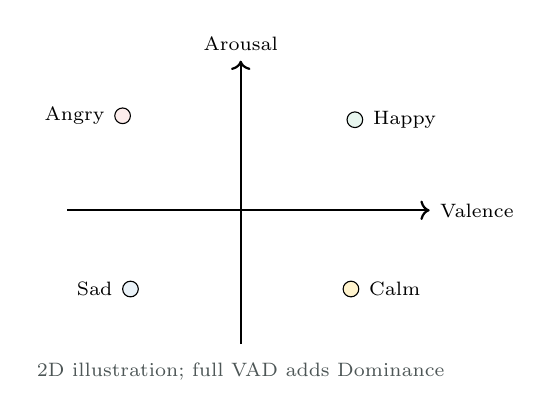
\begin{tikzpicture}[font=\scriptsize]
\draw[->,thick] (-2.2,0) -- (2.4,0) node[right]{Valence};
\draw[->,thick] (0,-1.7) -- (0,1.9) node[above]{Arousal};
\node[draw,circle,fill=SoftGreen,inner sep=2pt,label=right:{Happy}] at (1.45,1.15) {};
\node[draw,circle,fill=SoftGold,inner sep=2pt,label=right:{Calm}] at (1.4,-1.0) {};
\node[draw,circle,fill=SoftRed,inner sep=2pt,label=left:{Angry}] at (-1.5,1.2) {};
\node[draw,circle,fill=SoftBlue,inner sep=2pt,label=left:{Sad}] at (-1.4,-1.0) {};
\node[align=center,MutedGray] at (0,-2.05) {2D illustration; full VAD adds Dominance};
\end{tikzpicture}
\end{center}
\end{columns}
\begin{exampleblock}{Why it was interesting}
Continuous emotion values could drive avatar facial expressions smoothly, instead of switching between fixed emotion presets.
\end{exampleblock}
\note{Explain: this would change the task from classification to regression.}
\end{frame}

% 16
\begin{frame}[t]{Why the VAD-to-Avatar Idea Was Deferred}
\begin{columns}[T,onlytextwidth]
\column{0.48\linewidth}
\begin{block}{Potential value}
\begin{itemize}
  \item More expressive than seven fixed labels
  \item Supports emotion interpolation
  \item Useful for AR/VR avatars and rigged characters
  \item Connects affective computing to animation pipelines
\end{itemize}
\end{block}
\column{0.49\linewidth}
\begin{alertblock}{Why out of scope for RP2}
\begin{itemize}
  \item Requires mapping discrete labels to VAD coordinates
  \item Changes learning objective from classification to regression
  \item Needs avatar rigging or animation prototype
  \item Evaluation likely needs user studies on naturalness/believability
\end{itemize}
\end{alertblock}
\end{columns}
\vspace{0.25cm}
\keytake{We deferred this to keep RP2 to one measurable question: does cross-modal attention improve Egyptian Arabic emotion recognition?}
\note{This is important: it shows scoping discipline, not lack of creativity.}
\end{frame}

% 17
{\setbeamertemplate{footline}{}
\setbeamercolor{background canvas}{bg=DeepBlue}
\begin{frame}[plain]
\vspace{0.65cm}
\begin{center}
{\color{white}\LARGE\bfseries Conclusion}\\[0.55cm]
\end{center}
\begin{columns}[T,onlytextwidth]
\column{0.31\linewidth}
\begin{beamercolorbox}[rounded=true,sep=0.35cm,wd=\linewidth]{block body}
\textbf{Problem}\par
Egyptian Arabic emotion is multimodal, sarcastic, and under-resourced.
\end{beamercolorbox}
\column{0.31\linewidth}
\begin{beamercolorbox}[rounded=true,sep=0.35cm,wd=\linewidth]{block body}
\textbf{Proposal}\par
Tri-CAN replaces late fusion with text-driven cross-modal attention.
\end{beamercolorbox}
\column{0.31\linewidth}
\begin{beamercolorbox}[rounded=true,sep=0.35cm,wd=\linewidth]{block body}
\textbf{Experiment}\par
Compare against baselines using 5-fold CV, ablations, and sarcasm analysis.
\end{beamercolorbox}
\end{columns}
\vspace{0.65cm}
\begin{center}
{\color{AccentBlue!25!white}\Large Thank you - Questions?}\\[0.25cm]
{\color{white!70}\small Nour Gaser \quad \& \quad Mohamed Wael}
\end{center}
\note{Close with the three-part summary: problem, proposal, experiment.}
\end{frame}
\setbeamercolor{background canvas}{bg=white}
}

\end{document}
